\chapter{竞品与需求分析}
% 官方要求：结合往年比赛视频、其它学校开源资料、论坛等信息，分析其它学校机器人各项功能的完成度及技术水平，概述值得借鉴之处或者有待改进之处。

\section{综述：各校空中机器人技术水平概览}

根据往年比赛视频、各校开源资料及 RoboMaster 社区论坛信息，本赛季各高校空中机器人主要在悬停稳定性、轻量化、火力与可靠性四个方面展开竞争：
\begin{itemize}
    \item \textbf{悬停稳定性}：多数强队的空中机器人均搭载室内定位模块（光流、激光测距或雷达里程计），以保证空中稳定悬停；
    \item \textbf{轻量化}：深圳大学在 24 赛季即实现了空载（带电池）低于 \qty{13}{\kg} 的轻量化设计\cite{RM2024RobotPilotsSZ}，在 26 赛季空中机器人最大重量为 \qty{13}{\kg}（不含裁判系统）的限制下仍具备重量余量；
    \item \textbf{火力}：浙江大学、南昌大学\cite{RM2024PassionNCU}与辽宁科技大学\cite{RM2025CODLNUST}研发了三轴云台，在弹道、自瞄等方面较普通双轴云台表现更好，但会增加机身自重与不稳定性，故多数队伍未采用；
    \item \textbf{可靠性}：上海交通大学、中国科学技术大学、华南理工大学\cite{RM2025SCUTSouthChinaTiger}、东北大学等学校拥有一次空中支援稳定推掉敌方满血旋转前哨站的能力，但空中机器人整体故障率仍居高不下，作为最易受损的兵种，稳定性依然是各队最关注的核心问题。
\end{itemize}

\begin{figure}[hbtp!]
    \centering
    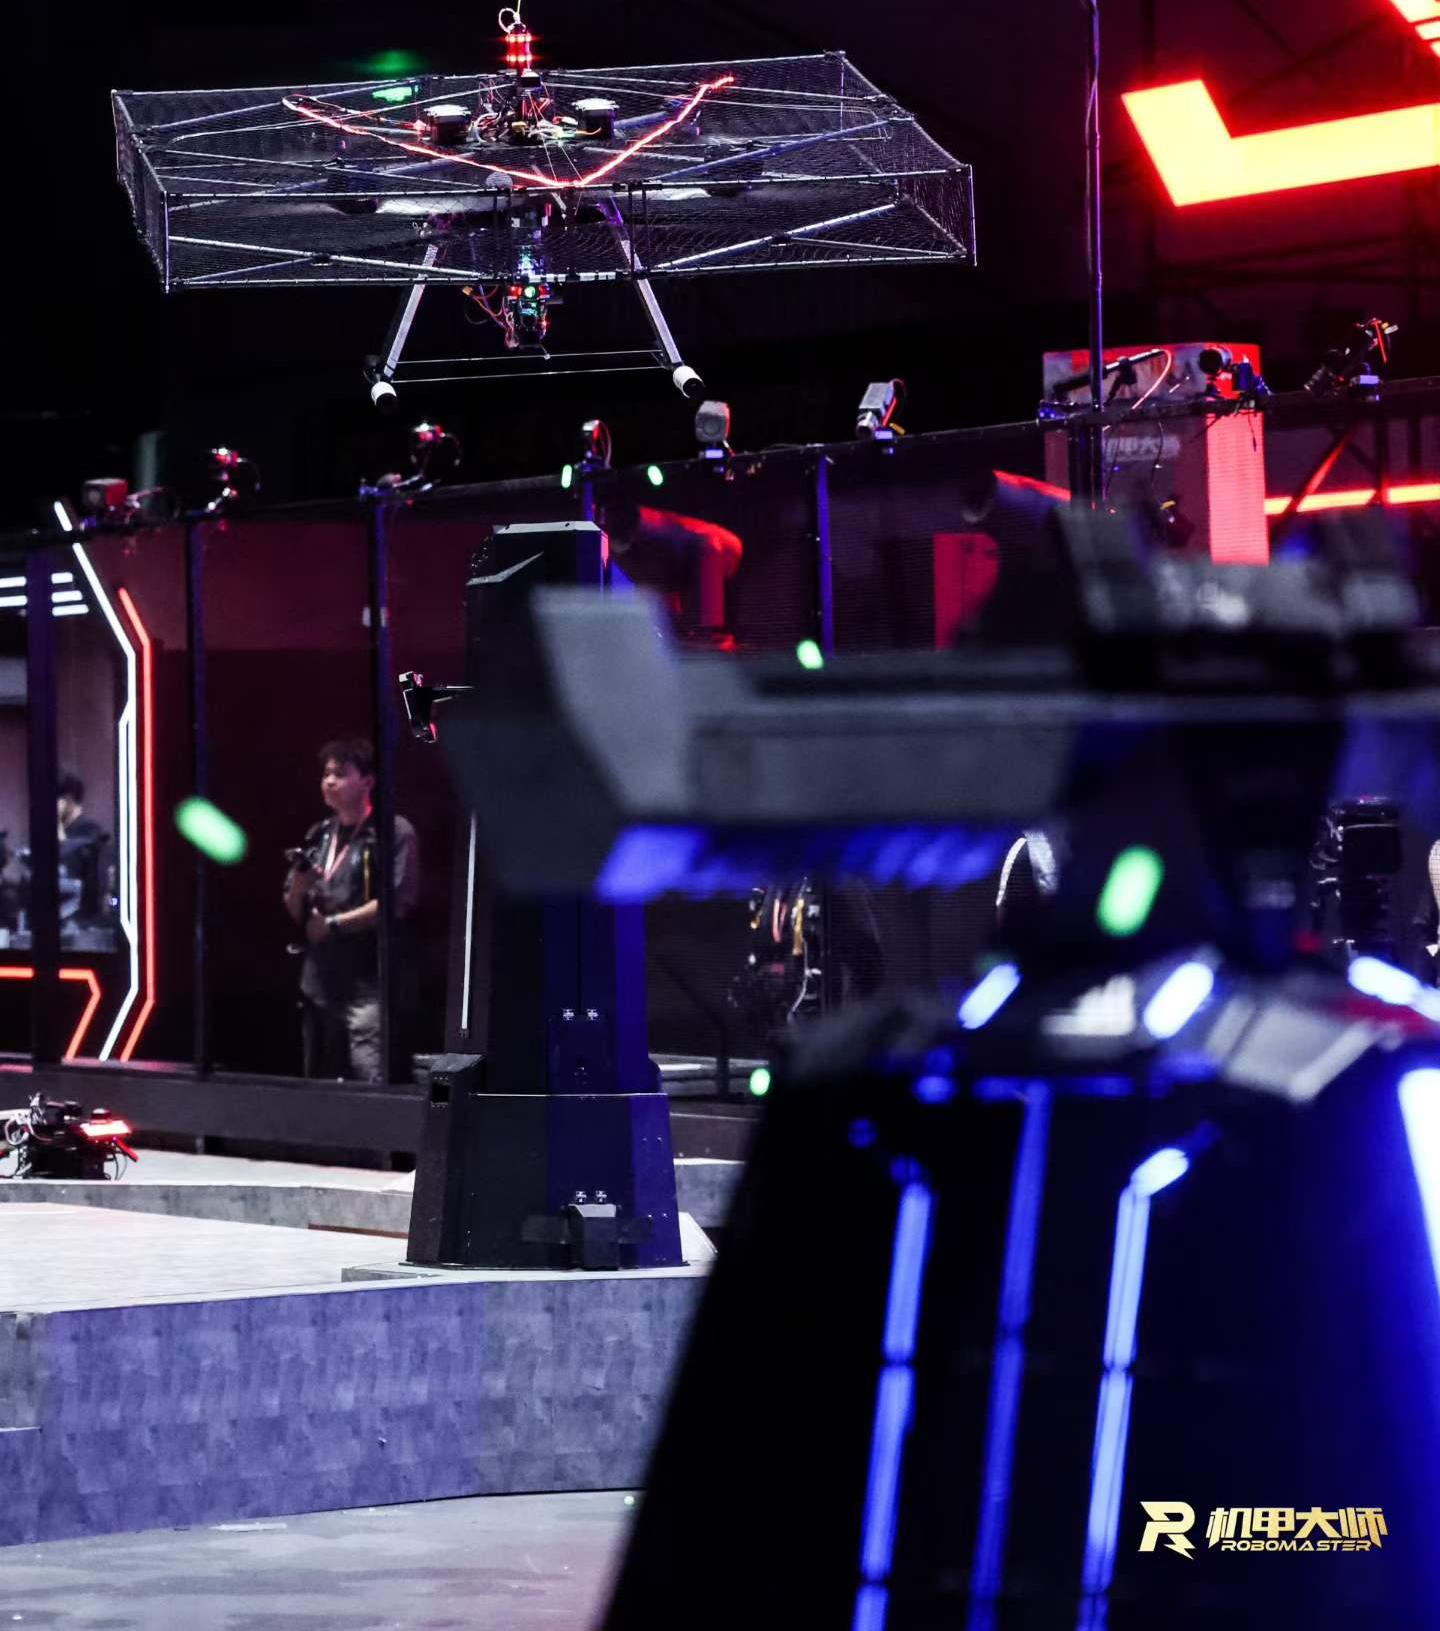
\includegraphics[width=0.78\linewidth]{figure/2_竞品与需求分析/2025赛季南部赛区空中机器人数据统计.png}
    \caption{2025 赛季超级对抗赛南部赛区各队空中机器人数据统计（图源：仲恺奇点战队开源报告\cite{zhongkai_qidian_drone_2026}）}
    \label{fig:竞品数据统计}
\end{figure}

\section{仲恺农业工程学院——奇点战队（穹隼）}

仲恺农业工程学院奇点战队在 2026 赛季开源了其"穹隼"空中机器人完整技术方案\cite{zhongkai_qidian_drone_2026}，其结构设计、动力系统与研发流程具有较强的参考价值。

\subsection{各项功能的完成度及技术水平}

\subsubsection{机械}
\begin{itemize}
    \item 构型：采用四轴 X 型布局、28 寸大桨盘，机架、机臂、弹仓、云台均作为可快拆子模块设计，实现高模块化；
    \item 动力：好盈 HM 8110 110KV 电机配合 28 寸桨叶与 XRotor Pro 60A 电调，悬停工况下单电机拉力约 \qty{5.1}{\kg}，整机总拉力满足满载（800 发弹丸）需求；
    \item 折叠桨保：采用一体式折叠桨保，配合机架折叠满足 \qty{1385}{\mm}$\times$\qty{1385}{\mm} 收纳尺寸，同时针对初版折叠处易松、强度不足的问题进行了多轮迭代；
    \item 供电与电池架：自制 DJI Matrice 4D 电池架（两并两串、\qty{48}{\V}），并配套电池缓启动模块，避免大电流冲击；
    \item 云台：GM6020 直驱 Yaw 轴、达妙 3507 驱动 Pitch 轴的小惯量二轴云台，内部采用鹅颈弹链（参考西安交大开源）与光固化树脂枪管，云台结构如\figref{fig:仲恺云台示意图}所示；
    \item 发射机构：M2006 拨弹盘配合 SUNNYSKY A2212 摩擦轮，实现 1000 发仅 1--3 发卡弹的供弹可靠性。
\end{itemize}

\begin{figure}[hbtp!]
    \centering
    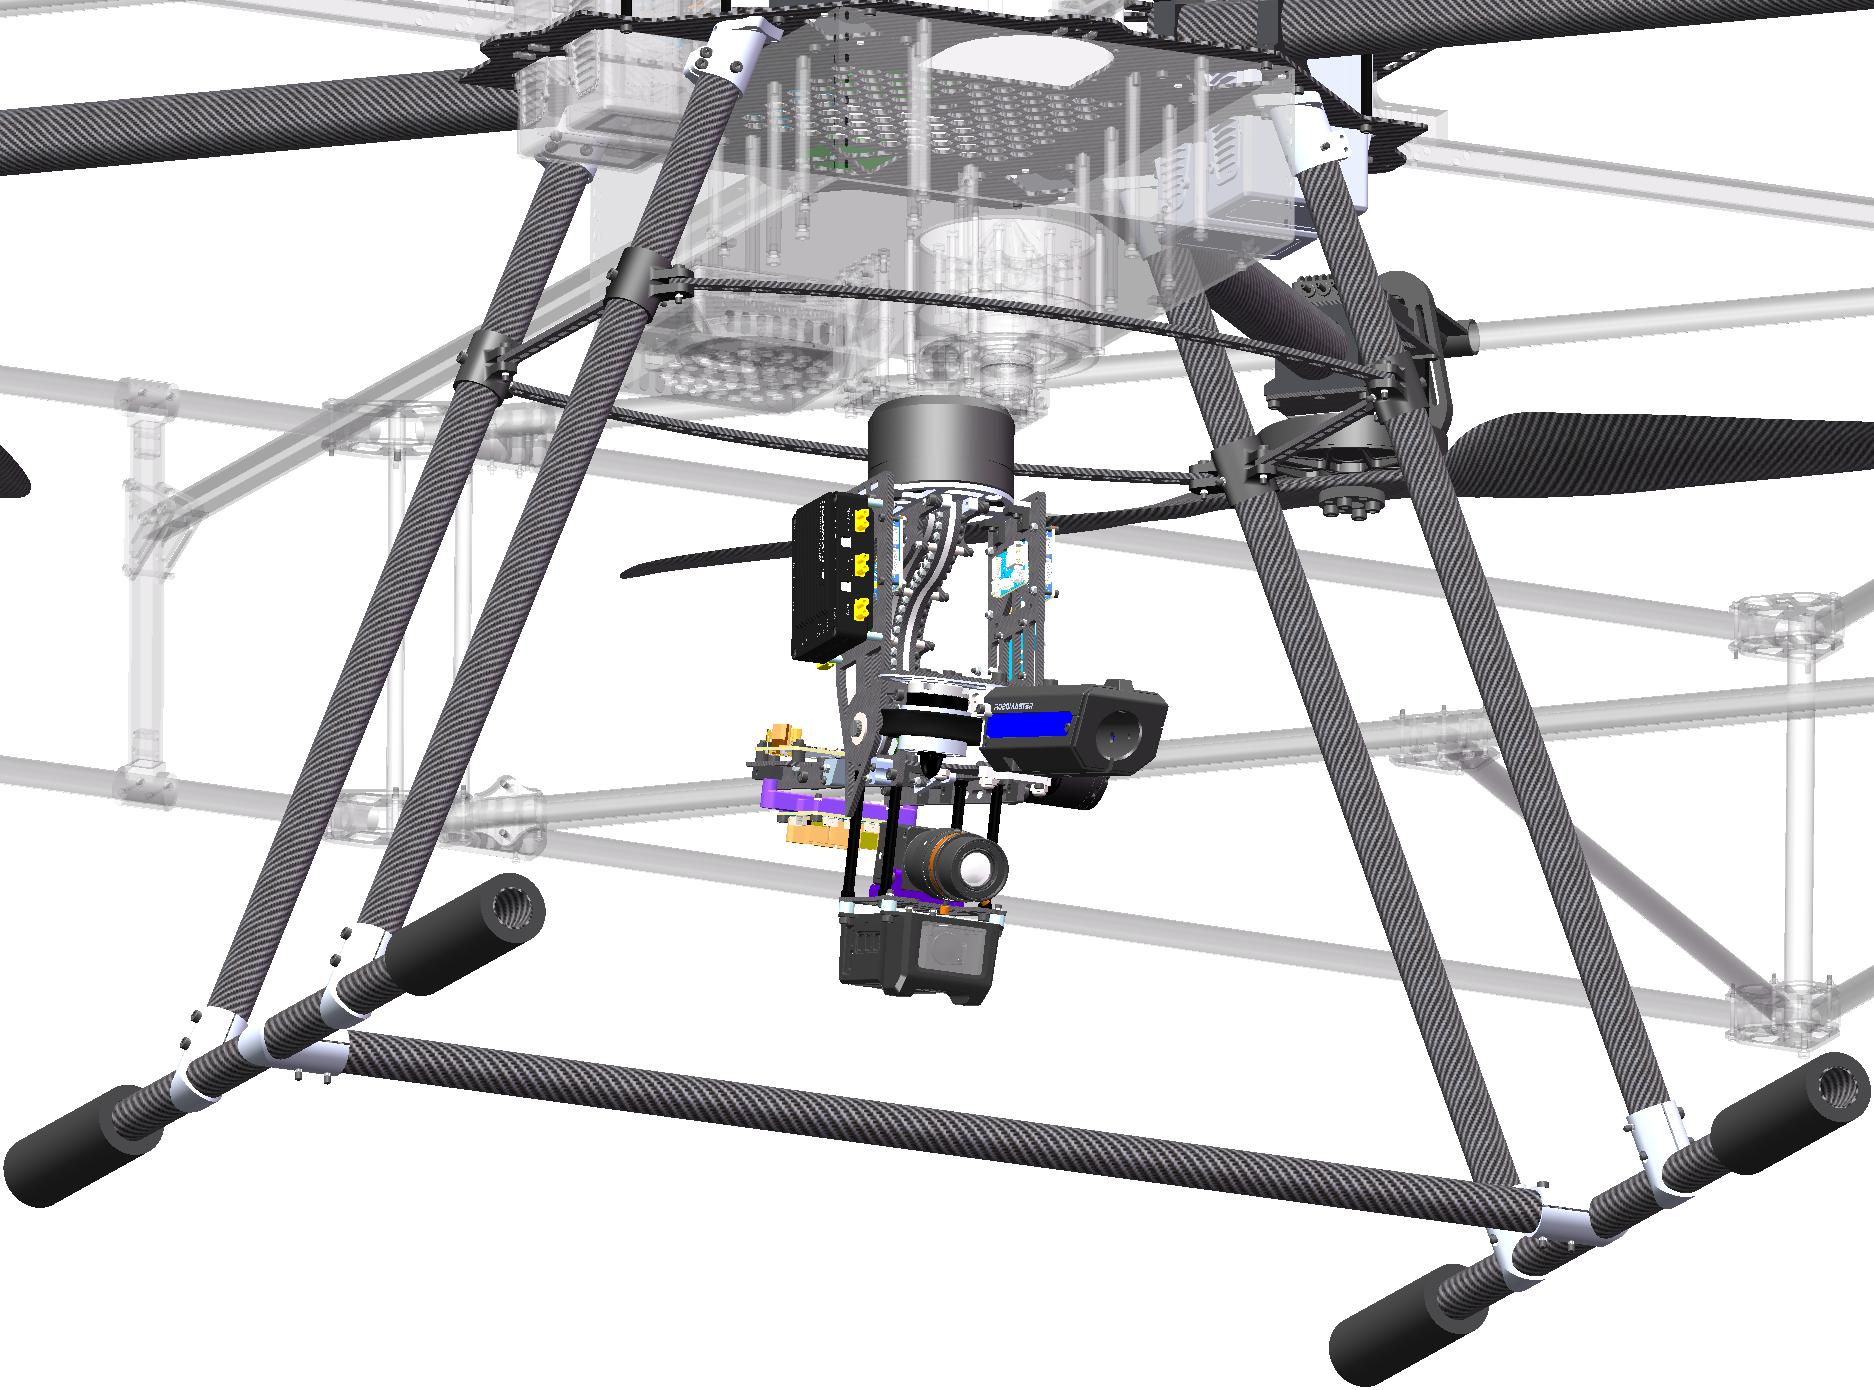
\includegraphics[width=0.7\linewidth]{figure/2_竞品与需求分析/仲恺奇点穹隼云台示意图.png}
    \caption{仲恺奇点穹隼空中机器人云台示意图（图源：仲恺奇点战队开源报告\cite{zhongkai_qidian_drone_2026}）}
    \label{fig:仲恺云台示意图}
\end{figure}

\subsubsection{电控与硬件}
\begin{itemize}
    \item 飞控采用 AC Fly A9 开源飞控，并复用上一赛季的室内定位方案（匿名光流 + TF mini 激光测距）；
    \item 电源系统自研 \qty{48}{\V} 电池缓启动、\qty{48}{\V} 转 \qty{24}{\V} 云台降压、NUC \qty{24}{\V} 转 \qty{19}{\V} 降压与 N630 发射电调模块。
\end{itemize}

\subsubsection{视觉与自瞄}
\begin{itemize}
    \item 自瞄系统搭载海康工业相机与 12mm 镜头，重构了决策器并引入精密火控算法；
    \item 测试中无火控 5m 旋转装甲板命中率约 51\%，加火控后命中率提升至 75\%，弹速稳定且散布控制在 5m 处 1/4 块装甲板以内。
\end{itemize}

\subsection{值得借鉴之处}
\begin{itemize}
    \item 以"需求 ID"驱动设计：对赛季规则进行量化拆解（弹丸伤害、经验收益、资源预算等），形成分级需求表，保证设计目标明确、可度量；
    \item 高模块化设计：机架、桨保、弹仓、云台均可快拆，便于检录、运输与维修，支撑高强度连续比赛；
    \item 自制电池架与缓启动模块：保障动力系统供电安全与稳定，避免炸机风险；
    \item 折叠桨保与轻量化：在满足收纳尺寸的同时兼顾强度，并给出了多轮迭代的工程经验。
\end{itemize}

\subsection{有待改进之处}
\begin{itemize}
    \item 空中机器人坠机率仍然较高，稳定性有待进一步提升；
    \item 云台弹速曾出现不稳定、散布随整机飞行放大等问题，自瞄命中率发挥不稳定；
    \item 折叠桨保初版折叠处易松动、连接处强度不足，依赖后续迭代改进。
\end{itemize}

\section{深圳技术大学——悍匠战队}

深圳技术大学悍匠战队开源了其 2026 赛季空中机器人的机械设计报告与经验分享\cite{sztu_hanjiang_drone_2026}，其"稳定为先"的设计理念与详细的复盘方法非常值得学习。

\subsection{各项功能的完成度及技术水平}

\subsubsection{机械}
\begin{itemize}
    \item 构型：四轴 X 型布局（如\figref{fig:深技大机架布局}所示），好盈 8110 电机配合 30 寸原装桨叶，并采用反桨（电机倒装）方案，让飞机获得完整下洗气流，提升力效、降低电池电流压力；
    \item 机架：重新设计的轻量化机架，配合供弹链路、雪橇型起落架与自制脚架电池架，兼顾强度与重心配置；
    \item 桨保：一体化折叠桨保，四角沿横向碳管上翻折叠以满足 \qty{1350}{\mm}$\times$\qty{1350}{\mm} 收纳尺寸，采用扎网封闭，展开便捷；
    \item 云台：Yaw 轴 GM6020 直驱、Pitch 轴 4310 电机连杆的小惯量二轴云台（如\figref{fig:深技大云台结构}所示），电机余量大、响应灵敏；发射机构沿用 3508 电机与平面摩擦轮方案，稳定可靠、研发经验丰富。
\end{itemize}

\begin{figure}[hbtp!]
    \centering
    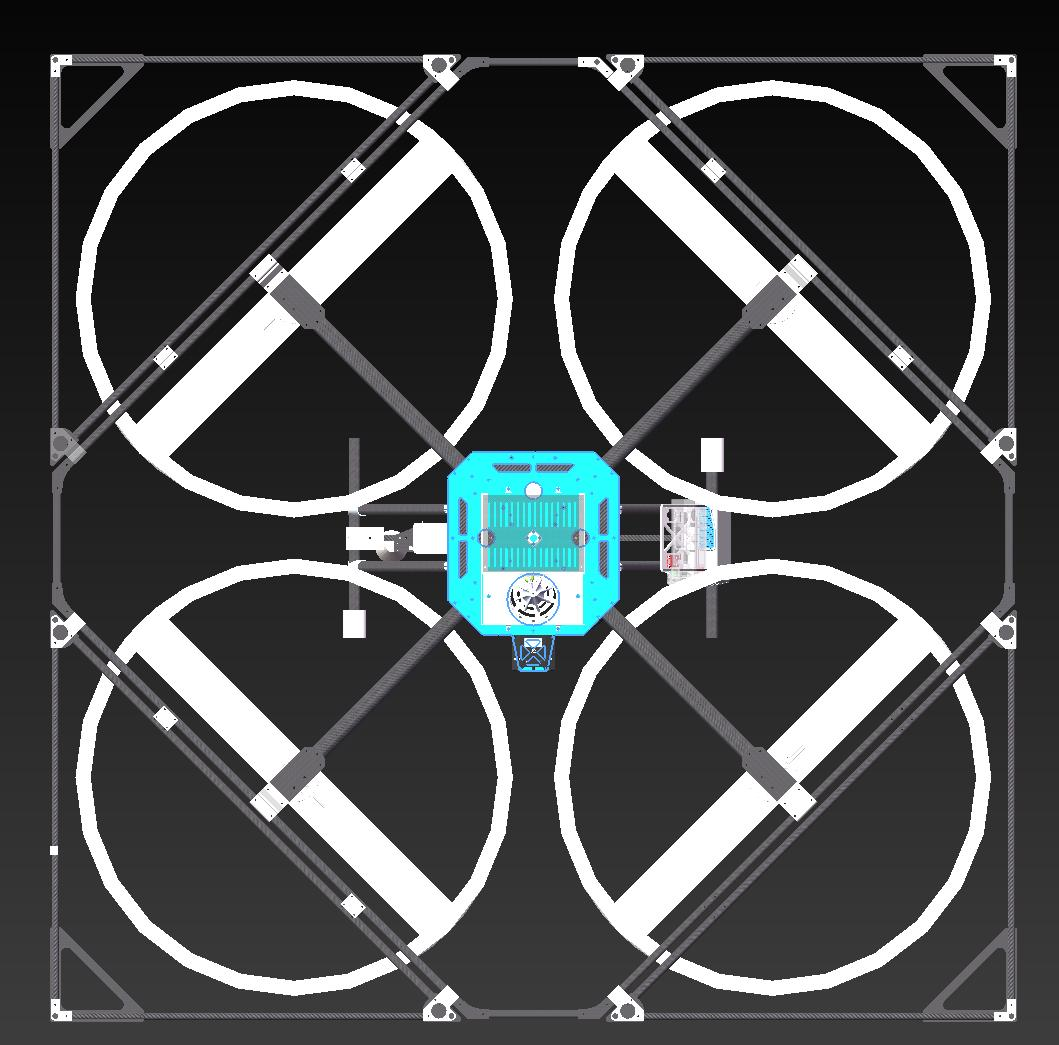
\includegraphics[width=0.66\linewidth]{figure/2_竞品与需求分析/深技大悍匠机架布局.png}
    \caption{深技大悍匠空中机器人机架布局（图源：深技大悍匠战队开源报告\cite{sztu_hanjiang_drone_2026}）}
    \label{fig:深技大机架布局}
\end{figure}

\begin{figure}[hbtp!]
    \centering
    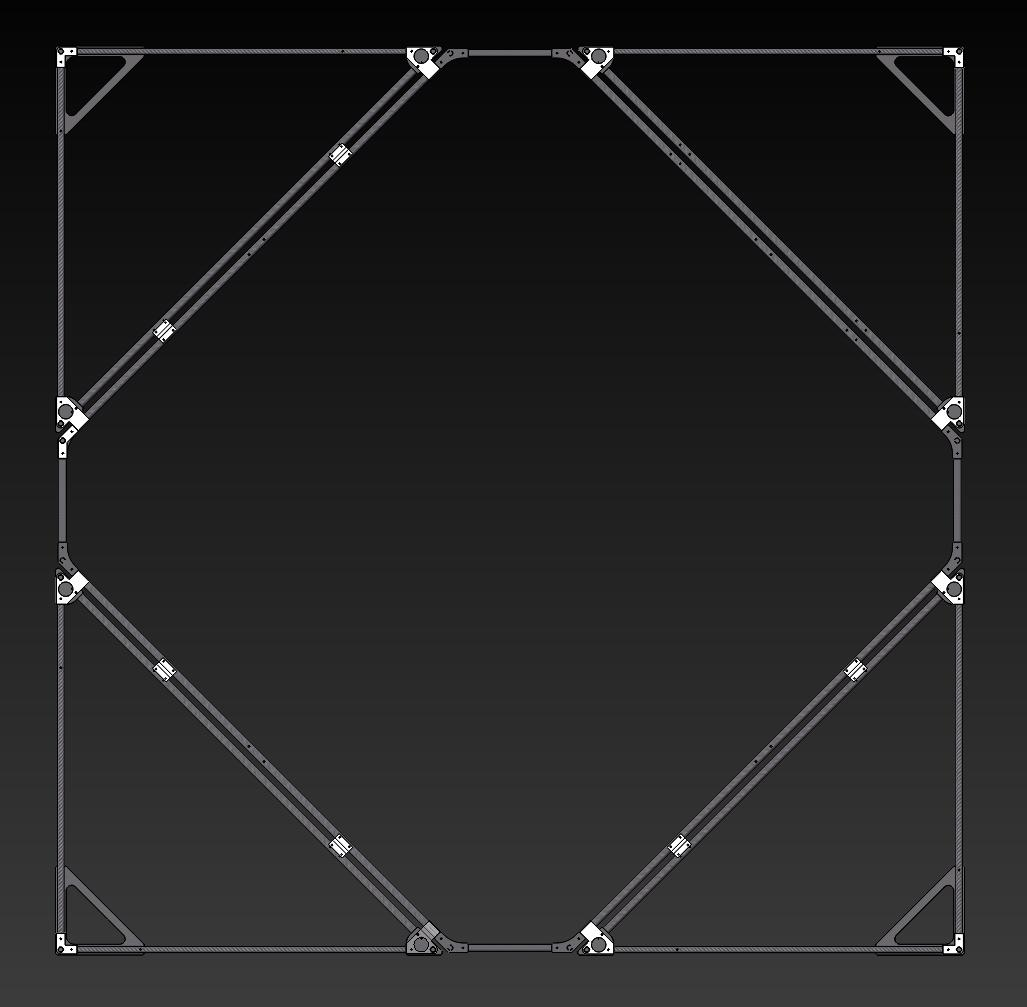
\includegraphics[width=0.66\linewidth]{figure/2_竞品与需求分析/深技大悍匠云台结构.png}
    \caption{深技大悍匠空中机器人云台结构（图源：深技大悍匠战队开源报告\cite{sztu_hanjiang_drone_2026}）}
    \label{fig:深技大云台结构}
\end{figure}

\subsubsection{电控与硬件}
\begin{itemize}
    \item 飞控采用 DJI A3，机载小电脑选用上科大 AX650N，并针对轻量化需求进行选型；
    \item 通过更换新电、自制电池架与缓启动模块，保障 BO3 完整起飞能力。
\end{itemize}

\subsubsection{视觉与定位}
\begin{itemize}
    \item 基于 guidance 定位系统（安装于雪橇起落架），保证定位视野内无机身组件干扰；
    \item 云台按视觉需求将发射装置与自瞄相机轴线贴近，提高命中一致性。
\end{itemize}

\subsection{值得借鉴之处}
\begin{itemize}
    \item 高度模块化：桨保 8 颗螺丝、电池架 4 颗螺丝、云台 6--8 颗螺丝即可拆卸，极大降低机械维护强度；配合 50 发小弹舱与调试架，可脱离整机进行电控视觉调试；
    \item 反桨方案：在尺寸与收纳限制下提升力效，减少桨保骨架对气流的阻挡，并给出了详细的电机倒装注意事项；
    \item 重心配置与起落架设计：综合考虑飞行稳定性与炸机时桨叶、电机的保护；
    \item 完善的复盘方法：对 25 赛季 H 型机架、桨保、电池布置等问题逐一复盘，指导新机重新设计。
\end{itemize}

\subsection{有待改进之处}
\begin{itemize}
    \item 轻量化能力相对薄弱，经历了漫长而痛苦的减重迭代过程，也给电控、硬件、视觉带来额外工作量；
    \item 高度模块化的副作用是各结构需单独固定，增加了不必要的重量；
    \item 3508 平面摩擦轮方案偏重，射击效果优于它的队伍普遍采用小电机 + 弧形摩擦轮。
\end{itemize}

\section{需求分析}

结合赛季规则、地形变化以及上述竞品的优劣分析，我们对本队空中机器人提出了明确的作战定位与功能需求。空中机器人在场上的任务包括：快速击打敌方前哨站、击杀敌方地面关键单位（工程、步兵、英雄）、开启能量机关、攻击敌方基地，以及阻止敌方地面单位进攻、为队友提供视野与火力支援。为满足上述任务，空中机器人必须具备：
\begin{itemize}
    \item 良好的悬停稳定性与充沛续航，保证空中视野与持续火力；
    \item 稳定的动力系统与充足的冗余，避免因动力不足或电池过流导致坠机；
    \item 高精度的自瞄与弹道系统，在 \qty{9}{\m} 距离上保持小装甲板内的散度；
    \item 大角度双轴云台，满足对前哨站、能量机关等不同目标的打击角度；
    \item 全场可靠的定位系统与"永不坠机"的多级安全保护。
\end{itemize}

据此，我们给出空中机器人的功能需求清单，如\tabref{tab:竞品需求清单}所示，并将需求落实到机械、电控、视觉各组的研发计划中。

\begin{longtable}[htbp!]{ m{1.9cm}<{\centering}  m{2.7cm}<{\centering}  m{1.3cm}<{\centering}  m{2.5cm}<{\centering}  m{6.4cm}<{\centering} }
\hline
需求ID & 功能需求 & 优先级 & 负责人 & 需求目标 \\
\hline
\endfirsthead
\hline
需求ID & 功能需求 & 优先级 & 负责人 & 需求目标 \\
\hline
\endhead
\hline
\multicolumn{5}{r}{接下页}
\endfoot
\caption{空中机器人功能需求清单}
\label{tab:竞品需求清单}
\endlastfoot
 \hline
 机组-001 & 强续航 & S & 机械 & 实战场景下飞行时间达到 7 分钟以上，动力系统稳定、抗干扰 \\
 \hline
 机组-002 & 定点定位 & S & 算法 & 搭载 GPS、Livox MID-360 雷达与激光检测模块，全场连续可靠定位 \\
 \hline
 机组-003 & 轻量化高强度 & S & 机械 & 碳纤维板主体结构，满足检录收纳尺寸与快速部署 \\
 \hline
 机组-004 & 折叠收纳 & S & 机械 & 机臂与桨保可折叠，折叠后满足检录收纳尺寸要求 \\
 \hline
 机组-005 & 弹道精度 & S & 机械/算法 & 高频顺畅发射不卡弹，\qty{9}{\m} 距离散度在小装甲板范围内 \\
 \hline
 机组-006 & 大角度云台 & S & 机械/电控 & Yaw 轴水平 $180^{\circ}$ 旋转，Pitch 轴满足近距离开启能量机关需求 \\
 \hline
 机组-007 & 安全可靠 & S & 算法/电控 & 多级安全保护与一键夺权机制，实现"安全飞行，永不坠机" \\
 \hline
\end{longtable}
